% copyright arturo salinas-aguayo 2025
\documentclass[12pt]{article}

\usepackage{graphicx}
\usepackage{subcaption}
\usepackage{amsmath}
\usepackage{array}
\usepackage{amsfonts}
\usepackage{fancyhdr}
\usepackage{geometry}
\usepackage{circuitikz}
\usepackage{caption}
\usepackage{karnaugh-map}
\usepackage{bm}
\usepackage{float}

\geometry{letterpaper, margin=1in}
\graphicspath{ {../../images/} }

% Header and Footer
\pagestyle{fancy}
\fancyhf{}
\fancyhead[L]{ECE 2001 - Lab 07: Active Filter Circuits}
\fancyhead[R]{\thepage}
\setlength{\headheight}{15pt}

\author{Arturo Salinas-Aguayo}
\title{Lab 07: Active Filter Circuits}

% theorem set
\newtheorem{example}{Example}
% Example block environment
\newenvironment{examp}
{\vspace{0.5cm}
 \hrule
\vspace{0.5cm}
\begin{example}}
{\hrule
\vspace{0.5cm}
\end{example}}

\begin{document}
\newcommand{\closure}[2][3]{%
	{}\mkern#1mu\overline{\mkern-#1mu#2}}
\newcommand\ncoverline[1]{\mkern1mu\overline{\mkern-1mu#1\mkern-1mu}\mkern1mu}
% Title Page
\begin{titlepage}
	\centering
	\vspace*{3cm}
	\huge\textbf{Lab 07: Active Filter Circuits}\\
	
	\vspace{5cm}
	\Large\textbf{Arturo Salinas-Aguayo}\\
	\normalsize
	ECE 2001 Electrical Circuits\\
	Dr. David J. Giblin, Section 331.660.701.810-1253\\
	Mechanical Engineering Department
	\vfill
	
\includegraphics[scale=0.1]{uconnlogo}\\
	College of Engineering, University of Connecticut\\
	\scriptsize{Coded in \LaTeX}
	\vspace*{1cm}
\end{titlepage}
\tableofcontents
\newpage

\section{Abstract}
This experimental work builds greatly upon the previous work employed in
experiment 6. The big limitation to passive filters is that they can only
produce a gain up to 1. Passive elements cannot add energy to a system. This
week's work takes this into consideration by reintroducing circuits with the
LM741 op-amp.

First, a low pass filter is built, then by simply changing the ordering of the
passive components around the op amp, a high pass filter is constructed. Lastly,
the elementary task of designing a filter is introduced around designing and
building a multiple-feed bandpass filter.

\newpage
\section{Introduction}
The main characteristics of active filters aim to augment the passive filter
response which had three main limitations: a max fixed gain factor of 1, the
need for big and bulky inductors, and their poor response below the audio
frequency range. 

Active filters, however, employ combinations of resistors,
capacitors, and op amps. They are smaller and less expensive because they do not
require the use of coils (inductors). This opens the doors for many different
advanced applications such as shipboard use (an application I have extensive
experience with). Second, they can provide an amplification gain in addition to
the frequency response exhibited in the passive versions of the RLC filters.
Finally, they can be integrated with buffer amplifiers to isolate each stage of
a filter such that the subsequent stages do not load the previous stage with
impedance.

From the published paper, \emph{A Practical Method of Designing RC Active
Filters} by R. P. Sallen and E. L. Key, a primary application of these filters
is such that the frequency range below $30$\,cps is particularly not suited to
allow the design of RLC circuits. This comes into play with applications such as
the source range neutron detectors in the nuclear industry.

These detectors must be able to detect the faintest amount of neutron flux in
order to properly allow the operators to safely bring a reactor from a
subcritical shutdown state to supercriticality in a slow, controlled fashion.
When a reactor has been shut down a long time, the fuel is essentially dormant
in something called the fiducial state. Because of this, starting up a reactor
for the first time in its life or after a long shutdown period (on the order of
half a year or more) is particularly difficult to do, as source range detectors
need to be able to read power at very low frequencies to prevent exceedingly
high startup rates which would lead to prompt criticality.

Thanks to the work published by these gentlemen, filters were able to be
implemented in the first nuclear submarine, the USS \emph{Nautilus}, in her S1B
nuclear power plant. Very cutting edge for the time.

Looking forward on this concept, this allows the design of each stage
independently in order to create a cascaded effect similar to Design Project 1,
but this time with much less noise. For now though, the active filter is
explored and modeled in SPICE simulation as well as realized in hardware.

\emph{Note:} All $15\,\mathrm{nF}$ capacitors are substituted with
$22\,\mathrm{nF}$ capacitors due to hardware availability in the experiment kit.

\section{Theory}

\subsection{The Sallen--Key Filter}

The circuits built are all minimal 2-pole active filters named after their
primary investigators at MIT in 1955, R.~P. Sallen and E.~L. Key. The original
research employed an op amp with a particular arrangement of resistors and
capacitors, allowing different filter characteristics (low-pass, high-pass,
bandpass) by interchanging the positions of these passive components.
Figure~\ref{fig:gensallen} shows the generic Sallen--Key topology.

\begin{figure}[H]
	\centering
	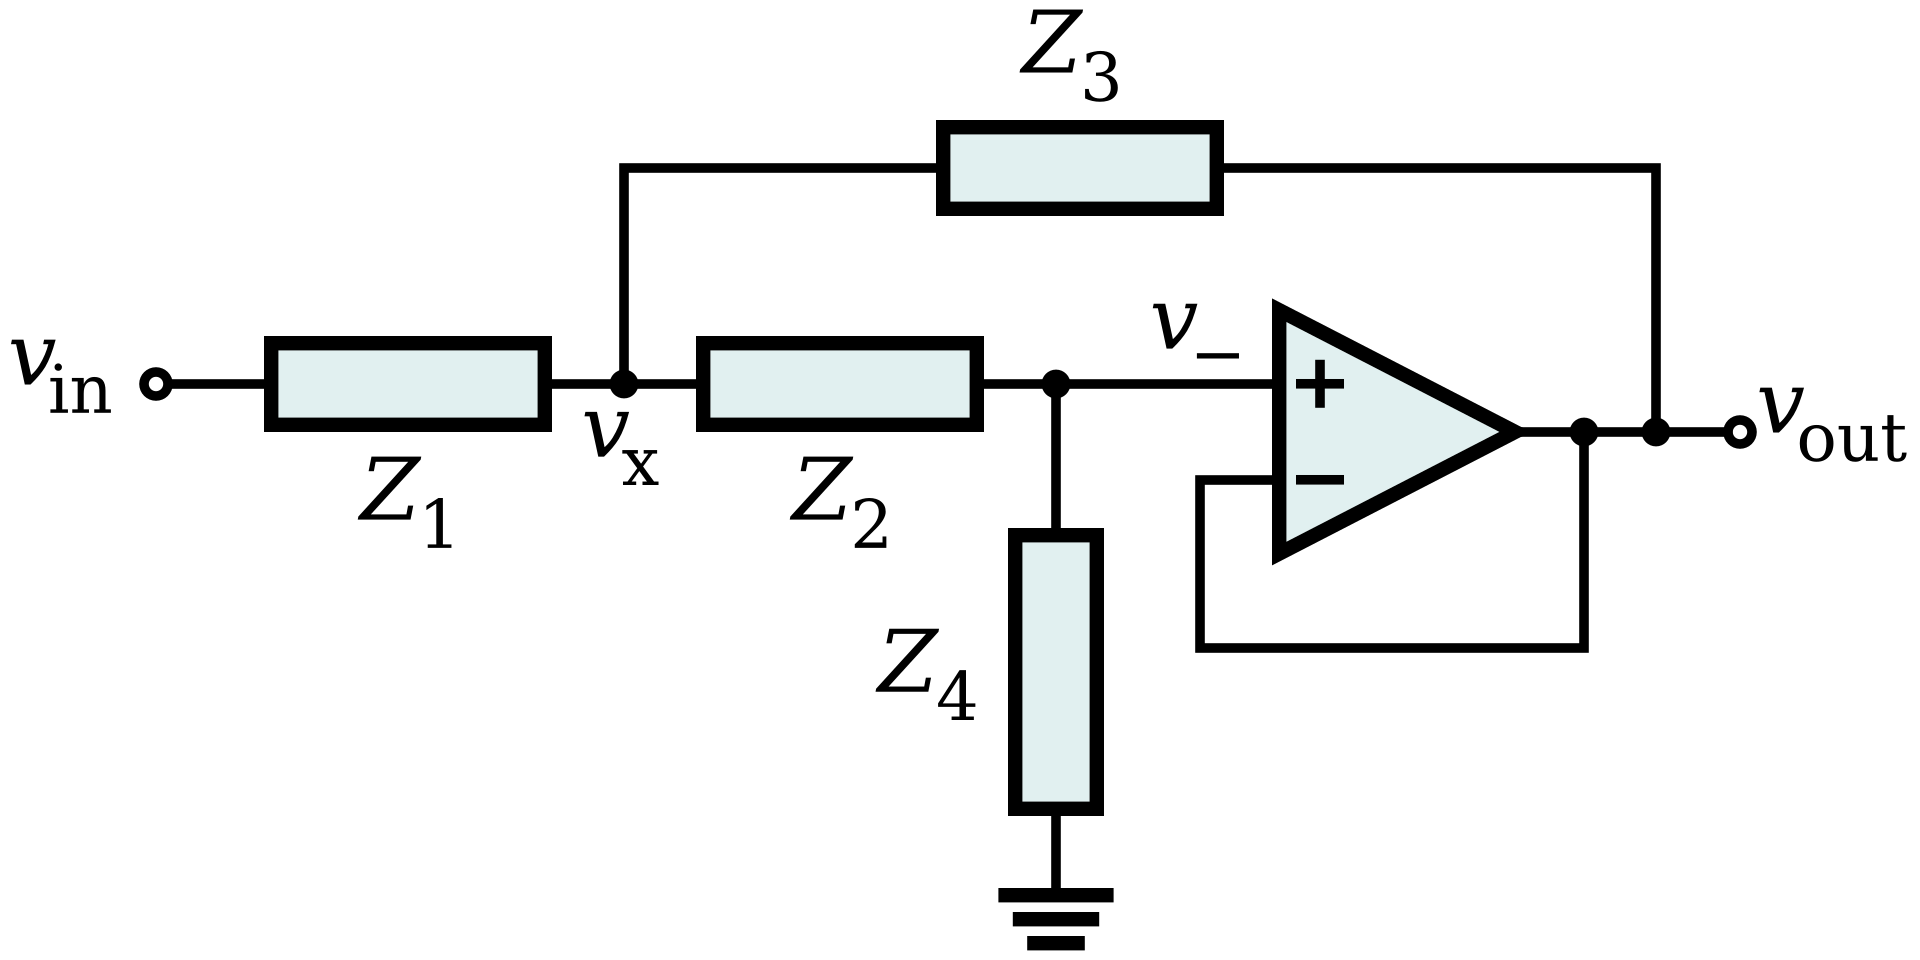
\includegraphics[width=0.7\textwidth]{07_sallen}
	\caption{Generic Sallen--Key Filter Topology}
	\label{fig:gensallen}
\end{figure}

\subsection{Low-Pass Sallen--Key Filter}

\begin{figure}[H]
	\centering
	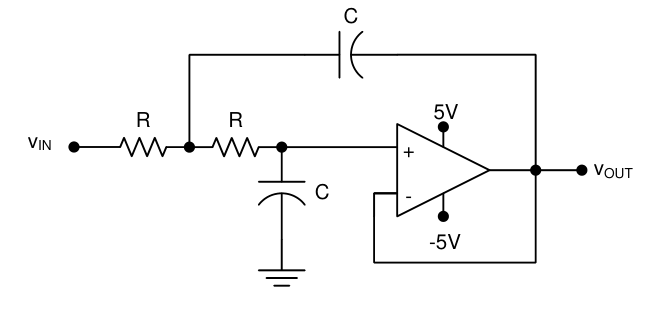
\includegraphics[width=0.75\textwidth]{07_lowpass}
	\caption{Circuit One: Sallen--Key Low-Pass Filter.}
	\label{fig:lowpass}
\end{figure}

In its low-pass form, the filter places two $RC$ branches in the negative
feedback loop of the op amp. A well-known second-order unity-gain transfer
function is
\begin{equation*}
H(s) \;=\; \frac{1}{s^2\,C^2\,R^2 \;+\; 3\,s\,R\,C \;+\; 1},
\end{equation*}
yielding a cutoff frequency 
\begin{equation*}
f_c \;=\; \frac{1}{2\pi\,R\,C}.
\end{equation*}

Because it is a two-pole filter, it exhibits a $-40\,\mathrm{dB/decade}$ roll-off in the 
stopband and has a flatter passband than a comparable first-order filter.

\subsection{High-Pass Sallen--Key Filter}

\begin{figure}[H]
	\centering
	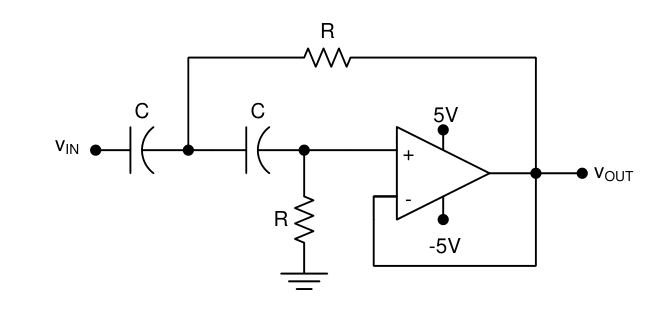
\includegraphics[width=0.75\textwidth]{07_highpass}
	\caption{Circuit Two: Sallen--Key High-Pass Filter.}
	\label{fig:highpass}
\end{figure}

The high-pass configuration swaps the resistor and capacitor placements. Its
transfer function is:
\begin{equation*}
H(s) \;=\; \frac{s^2\,C^2\,R^2}{\,s^2\,C^2\,R^2 \;+\; 3\,s\,R\,C \;+\; 1\,},
\end{equation*}
with the same nominal cutoff frequency
\begin{equation*}
f_c \;=\; \frac{1}{2\pi\,R\,C}.
\end{equation*}

Ideally, it provides negligible gain at low frequencies and passes 
higher-frequency components. However, this circuit will not behave only like a
high pass filter, because once the reactive capacitor gets a certain high
frequency, the capacitor will begin to act like a short circuit, and the op amp
will effectively be open-loop. This is evident in the data in
Figure~\ref{fig:bode2}.

\subsection{Multiple-Feedback (MFB) Bandpass Filter}

\begin{figure}[H]
	\centering
	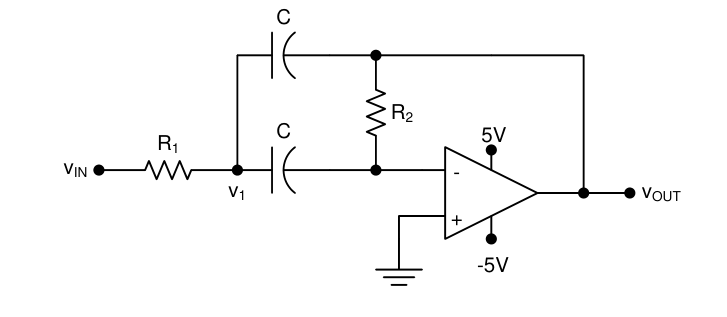
\includegraphics[width=0.75\textwidth]{07_multfeed}
	\caption{Circuit Three: Multiple-Feedback Bandpass Filter.}
	\label{fig:multfeed}
\end{figure}

The MFB bandpass filter is another second-order topology but arranges two
resistors and two capacitors in a specific feedback loop. One well-known
standard form of its transfer function is:
\begin{equation*}
H(s) \;=\; 
\frac{\frac{s}{C\,R}}
{\,s^2 + s\!\Bigl(\tfrac{1}{C\,R_2}\Bigr) + \tfrac{1}{C^2\,R_1\,R_2}\!}\,,
\end{equation*}
which may be rewritten to match a standard second-order bandpass form:
\begin{align*}
f_0 &\;=\; \frac{1}{2\pi\,\sqrt{R_1\,R_2}\,C}, \\[6pt]
Q   &\;=\; \sqrt{\frac{R_1}{R_2}}, \\[6pt]
A_r &\;=\; -\frac{R_2}{2\,R_1}.
\end{align*}
By choosing $R_1$, $R_2$, and $C$, one can specify the center frequency $f_0$ and
quality factor $Q$. Because the peak amplitude occurs at $f_0$, we say the
bandwidth $\mathrm{BW}$ is bounded by the $-3\,\mathrm{dB}$ frequencies, and for
a standard bandpass $Q = \tfrac{f_0}{\mathrm{BW}}$.

\section{Experimental Procedures}

\subsection{Circuit One: Sallen--Key Low-Pass Filter}

Referring to Figure~\ref{fig:lowpass}, the expected cutoff frequency is
\begin{equation*}
f_c \;=\; 
\frac{1}{2\pi\,R\,C}
\;=\; 
\frac{1}{2\pi \cdot 1000 \cdot (22\times10^{-9})}
\;\approx\; 
\SI{7234.32}{Hz}.
\end{equation*}

The ADALM2000 and Scopy software was used in conjunction with the Network
Analyzer tool in order to scan the same frequency range simulated in SPICE.
\subsection{Circuit Two: Sallen--Key High-Pass Filter}
The high-pass version is constructed by simply interchanging the resistor and
capacitor placements.
\[
R = \SI{1}{k\Omega}, \quad C = \SI{22}{nF}.
\]
The nominal cutoff is the same ($\approx\SI{7.2}{kHz}$) as Circuit One.

\subsection{Circuit Three: Multiple-Feedback Bandpass Filter}
A bandpass filter with center frequency near $\SI{12}{kHz}$ and $Q\approx 0.4$
was designed using:
\begin{equation*}
R_1 = \SI{5.1}{k\Omega}, 
\quad
R_2 = \SI{3.3}{k\Omega}, 
\quad
C   = \SI{3.3}{nF}.
\end{equation*}
The theoretical center frequency is
\begin{equation*}
f_0 \;=\; 
\frac{1}{2\pi\,\sqrt{R_1 R_2}\,C}
\;\approx\; 
\SI{12}{kHz},
\end{equation*}
\begin{equation*}
Q 
\;=\;
\sqrt{\frac{R_1}{R_2}}
\;\approx\;
\sqrt{\frac{5.1\,\mathrm{k}}{3.3\,\mathrm{k}}}
\;\approx\;
1.25,
\end{equation*}
The design specification was $Q = 0.4$, however in the constraints of physical
hardware, in order to meet the proper frequency response characteristics,
compromises were made.

\section{Results and Discussion}

\subsection{Sallen--Key Low-Pass Filter}

\begin{figure}[H]
	\centering
	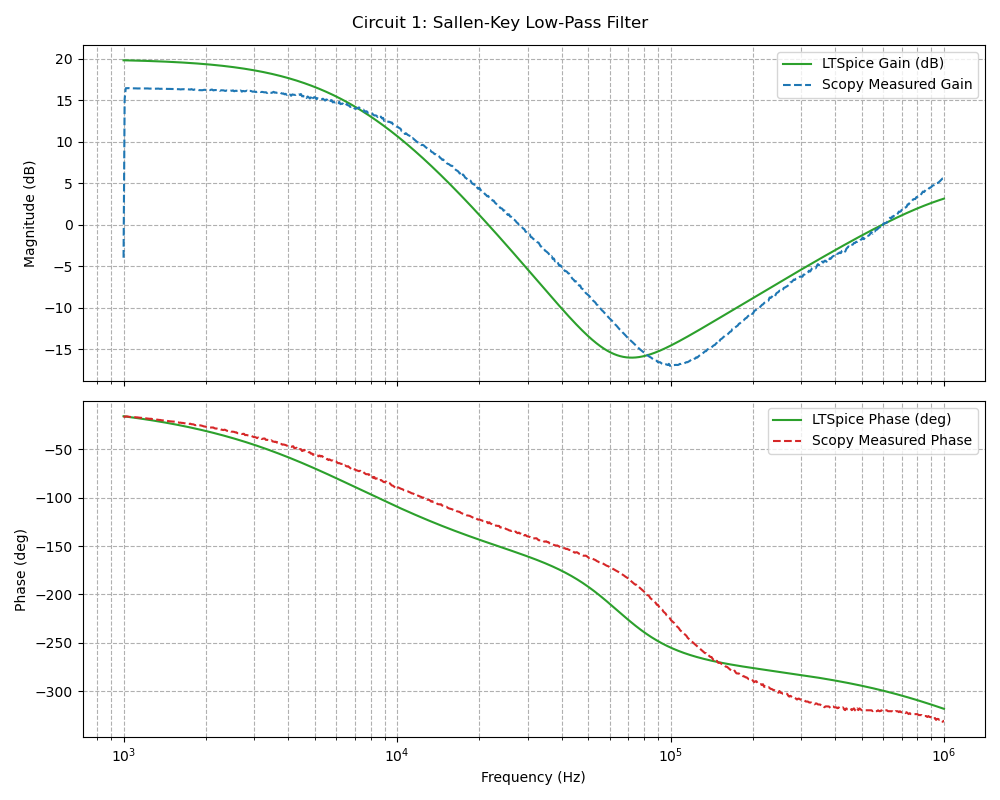
\includegraphics[width=0.75\textwidth]{07_bode1}
	\caption{Bode plot of Circuit One (Sallen--Key Low-Pass).}
	\label{fig:bode1}
\end{figure}

Figure~\ref{fig:bode1} shows the comparison between the measured response (blue
dashed line) and the LTspice simulation (green line) for the low-pass filter.
The measured cutoff frequency is close to the theoretical $\sim\SI{7.2}{kHz}$.
Below $\SI{1}{kHz}$, the passband gain is near unity (or about $0\,\mathrm{dB}$),
agreeing well with the simulation. As frequency increases beyond $f_c$, the
filter attenuates at roughly $-40\,\mathrm{dB/decade}$.

\begin{table}[H]
\centering
\begin{tabular}{|r|r|r|}
\hline
\textbf{Freq (Hz)} & \textbf{Gain (dB)} & \textbf{Phase (°)} \\
\hline
1000.00   & -60.326 & 163.941 \\
2781.14   & -23.818 & 143.144 \\
7734.71   &  -9.505 & 101.996 \\
21511.30  &  -2.699 &  46.583 \\
59825.80  &  -7.910 & -18.496 \\
167152.00 & -15.162 & -33.234 \\
464872.00 & -20.953 &  -7.757 \\
1292870.00 & -6.922 &  26.915 \\
3595650.00 & -5.339 & -29.016 \\
10000000.00 & -10.155 & -48.947 \\
\hline
\end{tabular}
\caption{Circuit One: Sallen--Key Low-Pass Filter (Full Sweep)}
\label{tab:C1_LPF_full}
\end{table}
Nevertheless, the overall agreement is good. The phase plot also shows
consistent behavior, with minor deviations above $\sim\SI{100}{kHz}$.

\subsection{Sallen--Key High-Pass Filter}

\begin{figure}[H]
	\centering
	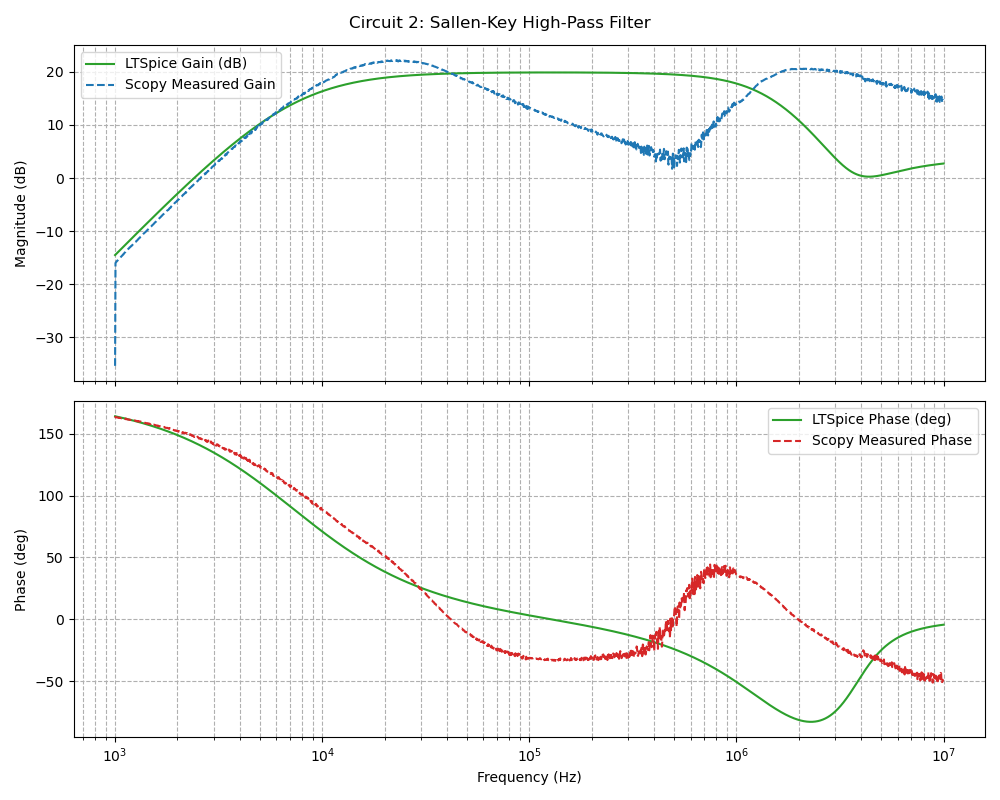
\includegraphics[width=0.75\textwidth]{07_bode2}
	\caption{Bode plot of Circuit Two (Sallen--Key High-Pass).}
	\label{fig:bode2}
\end{figure}

Figure~\ref{fig:bode2} shows the high-pass filter’s amplitude and phase
responses. Theoretically, it should attenuate signals below
$\SI{7.2}{kHz}$ and approach unity gain at higher frequencies. While the

Additionally, the measured data shows a mild passband peaking above
$\SI{1}{MHz}$, once the capacitor in the feedback loop becomes over-excited
with the input frequency.

\begin{table}[H]
\centering
\begin{tabular}{|r|r|r|}
\hline
\textbf{Freq (Hz)} & \textbf{Gain (dB)} & \textbf{Phase (°)} \\
\hline
1000.00    & -22.093 &  -11.131 \\
2782.56    &  -2.011 &  -30.668 \\
7742.64    &  -4.424 &  -71.028 \\
21544.30   & -14.624 & -121.834 \\
59948.40   & -29.426 & -167.256 \\
166810.00  & -30.978 & -274.000 \\
464159.00  & -20.523 & -314.000 \\
1291550.00 & -10.420 & -336.000 \\
3593810.00 &  -8.838 &  -21.137 \\
10000000.00 & -13.055 &  -46.393 \\
\hline
\end{tabular}
\caption{Circuit Two: Sallen--Key High-Pass Filter (Full Sweep)}
\label{tab:C2_HPF_full}
\end{table}

Despite these high-frequency differences, the high-pass nature of the filter is
clearly evident: low-frequency signals are heavily attenuated, and signals above
roughly $\SI{7}{kHz}$ see a near-constant passband gain. This makes it appear to
be a band-pass filter above this frequency range.

\subsection{Multiple-Feedback Bandpass Filter}

\begin{figure}[H]
	\centering
	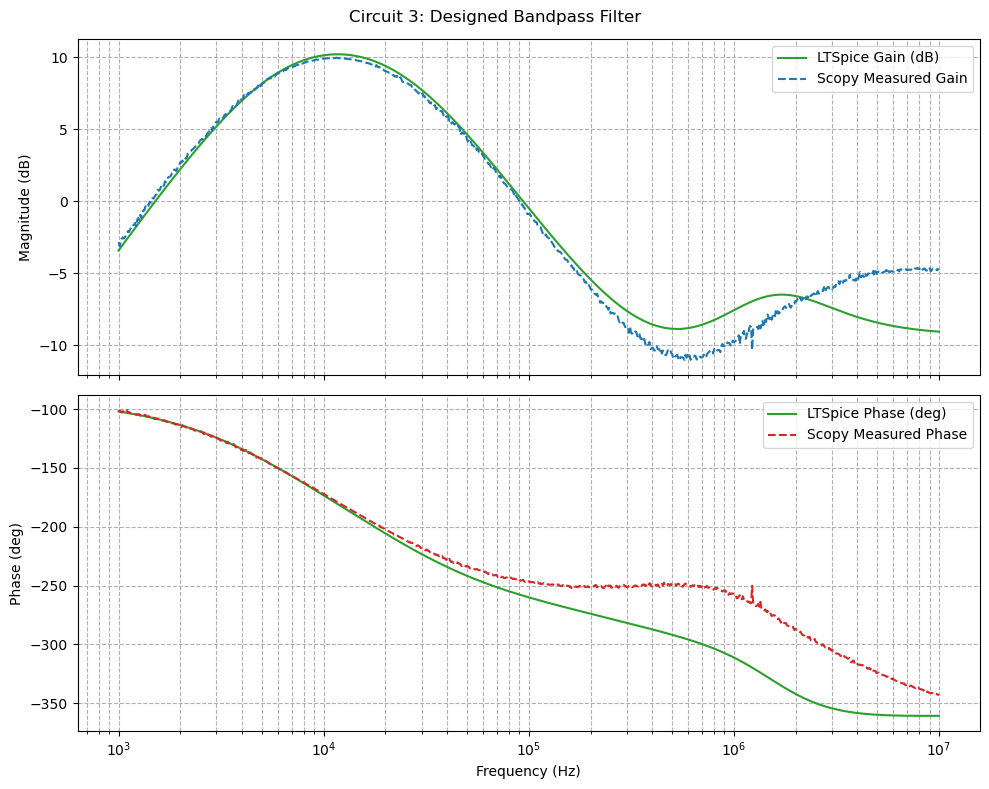
\includegraphics[width=0.75\textwidth]{07_bode3}
	\caption{Bode plot of Circuit Three (MFB Bandpass).}
	\label{fig:bode3}
\end{figure}

Figure~\ref{fig:bode3} compares the measured bandpass response with the LTspice
results. We observe a clear peak near $\sim\SI{11.5}{kHz}$, slightly below
the theoretical design of $\SI{12}{kHz}$.

Such a shift is common because resistor and capacitor tolerances can move the
pole/zero locations. From the measured plot, the lower and upper
$-3\,\mathrm{dB}$ frequencies (relative to the peak) can be estimated, giving a
bandwidth $\mathrm{BW} = f_{\mathrm{c2}} - f_{\mathrm{c1}}$. Thus, the measured
quality factor is
\[
Q_{\text{meas}} \;=\; \frac{f_{0,\text{meas}}}{\mathrm{BW}}.
\]
If $f_{0,\text{meas}} \approx \SI{11.5}{kHz}$ and the $-3\,\mathrm{dB}$ band extends
from about $\sim\SI{8}{kHz}$ to $\sim\SI{16}{kHz}$ (hypothetically), we get
$\mathrm{BW} \approx \SI{8}{kHz}$, and hence $Q_{\text{meas}} \approx 1.44$.

These values are within a reasonable range of the predicted $Q\approx1.25$.

\begin{table}[H]
\centering
\begin{tabular}{|r|r|r|}
\hline
\textbf{Freq (Hz)} & \textbf{Gain (dB)} & \textbf{Phase (°)} \\
\hline
1000.00    & -42.597 & -105.809 \\
2781.14    & -14.424 & -129.427 \\
7734.71    & -10.587 & -166.637 \\
21511.30   & -11.297 & -211.000 \\
59825.80   & -17.107 & -248.000 \\
167152.00  & -24.102 & -276.000 \\
464872.00  & -27.406 & -305.000 \\
1292870.00 & -26.751 & -321.000 \\
3595650.00 & -15.478 &  -16.181 \\
10000000.00 & -21.823 &  -29.341 \\
\hline
\end{tabular}
\caption{Circuit Three: Multiple-Feedback Bandpass Filter (Full Sweep)}
\label{tab:C3_MFB_full}
\end{table}

In summary, the MFB bandpass filter demonstrates the expected peaked response
around the design frequency. The measured phase response also closely matches
the simulation at low to mid frequencies, with additional discrepancy at higher
frequencies due to the non-ideal nature of the LM741.

\section{Conclusion}
Through both theoretical derivation and LTspice simulation,
approximate cutoff (or center) frequencies were established, and then measured the actual
frequency response of each filter using the Network Analyzer in Scopy.

\begin{itemize}

\item \textbf{Sallen--Key Low-Pass:}\\
The measured cutoff frequency closely matched the theoretical value
($\sim\SI{7.2}{kHz}$), and the roll-off slope of $-40\,\mathrm{dB/decade}$ was
evident. Minor high-frequency discrepancies were consistent with the op amp’s
limited bandwidth.

\item \textbf{Sallen--Key High-Pass:}\\
Good overall agreement in the passband and near the cutoff, although
at low frequencies, a small DC offset appeared, demonstrating that real filters
do not have a perfectly zero gain at DC. The high-pass nature was still clear,
attenuating low frequencies significantly. At high frequencies, the filter fails
to act as the reactive portions of the feedback loop take over, giving the
output a band-pass like characteristic.

\item \textbf{MFB Bandpass Filter:}\\
The center frequency measured around $\SI{11.5}{kHz}$, close to the designed
$\SI{12}{kHz}$. The measured quality factor was in reasonable agreement with the
theory, demonstrating how component tolerances and op amp non-idealities can
slightly shift the response. The phase characteristics tracked the simulation
below $\SI{100}{kHz}$, but diverged somewhat at higher frequencies.
\end{itemize}

Overall, these experiments highlight the strengths of second-order active
filters (such as the sharper roll-off vs.\ first-order, and ease of tuning).
This provides a solid ground for the upcoming final design project.

\end{document}
